\documentclass[11pt, sigconf]{acmart}
\usepackage{lipsum}
\usepackage{graphicx}
\begin{document}
\title{Recidivism Final Project Report}
\author{Andi Zhao, Helen Wu, Ryan Sun}
\date{\today}
\begin{abstract}
In a situation where algorithms dictate the future of humanity, one must proceed with extreme caution. For example, COMPAS, a software that is employed by the legal system to predict the recidivism rate of criminals, came under fire for neglecting the aspect of fairness in 2016. The ProPublica organization discovered racial bias within the predicted results, indicating a lack of thought and consideration of ethics while creating the algorithm. Using a dataset from the Iowa state government correctional center website, our final project focuses on this subject matter by attempting to predict recidivism with and without eliminating protected features from the training set to see if it has any effect on predicting recidivism. Pre-processing was required to eliminate unnecessary features and missing information. This report will detail the process in which we gathered and processed the data, as well as the conclusions that we drew from comparing our different models. 
\end{abstract}
\settopmatter{printacmref=false}
\setcopyright{none}
\renewcommand\footnotetextcopyrightpermission[1]{}
\pagestyle{plain}
\maketitle

\section{Motivation and Objective}
\hspace{5mm}In recent years, the traditional justice system has been accused of being biased to minority populations. In an attempt to resolve this issue, researchers developed \emph{COMPAS} (Correctional Offender Management Profiling for Alternative Sanctions), a tool used to circumvent the need for human judgement. The reason that it came under fire was because it was yielding biased results where “blacks are almost twice as likely as whites to be labeled a higher risk but not actually re-offend”\cite{1}. In addition, privacy and fairness have been at the forefront of modern artificial intelligence research. Some researchers have attempted to train models without protected attributes to avoid lawsuits. We wondered if eliminating protected attributes from the training set actually has any effects on the accuracy and precision of the model. If the protected attribute has no effect on the accuracy of the model, it would mean that either race has no effect on the outcome of the model or that race was predicted. On the other hand, if race does have an effect, it would mean that the researchers were correct to hide the protected attribute. 


Our intention is to use Iowa’s recidivism dataset to train a model with and without race as one of its features to determine if race is a factor in determining recidivism. We also attempt to predict race from recidivism data to see whether or not the results are significant enough to associate race and recidivism. Our plan was to train two models, one with logistic regression and the other with decision trees, to compare accuracy,  and other statistics.  The goal of this project is to produce models that predict with similar accuracies to that of COMPAS, as well as to uncover the relationship between using race as a feature and the corresponding results for predicting recidivism risk scores.

\section{Ethical Issues}

\hspace{5mm}The ProPublica study showcased the dangers of algorithmic decision making without concern for ethics, namely race, which can be detrimental to a true understanding and accurate modeling of recidivism. Additionally, the institutional biases within the COMPAS algorithm directly affects our  justice system because COMPAS risk scores are actually considered by judges during sentencing in certain US states. The chart below shows the flaws and clear biases of blindly using the COMPAS assessment to identify risk scores for an individual during sentencing.  
\begin{figure}[h] 	
\centering
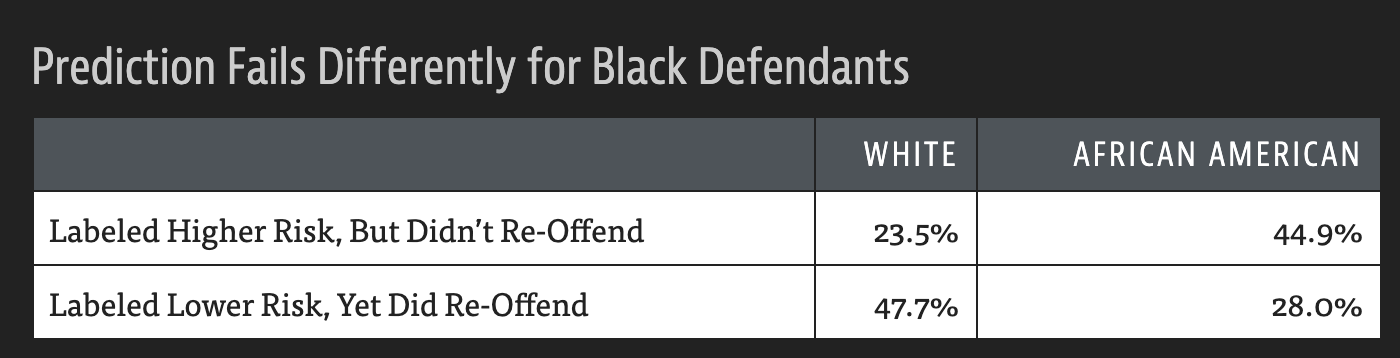
\includegraphics[width=3.3in]{asdf.png}
\caption{ProPublica's discovery}
\end{figure}


In our study, we are primarily concerned about whether or not using race as a feature will affect the prediction of recidivism for an individual. By including and excluding race as an attribute, we are able to create different models and compare their results, thus allowing us to determine whether or not race was a significant factor in the predictions.


\section{Domain and Dataset}


Describe your domain or data. If you had to do any data gathering, cleaning, preprocessing, etc., describe.

The dataset we chose to work with comes from the Iowa state’s government correctional center website. The reason we chose this one is because it has a large enough sample size, and is similar to that of COMPAS' , containing recidivism information for 26,000 individuals from 2007-2013. The recidivism (titled ‘Return to Prison’) column is determined whether the individual recidivated within the last 3 years.

We first created visualizations to look for any data inconsistencies and possible skews with the data set. We removed rows where the ethnic group values were incomplete (i.e., ‘White -’, ‘Black -’, ‘NA -’). In addition, we also removed any rows with missing values.

\begin{figure}[h] 	
\centering
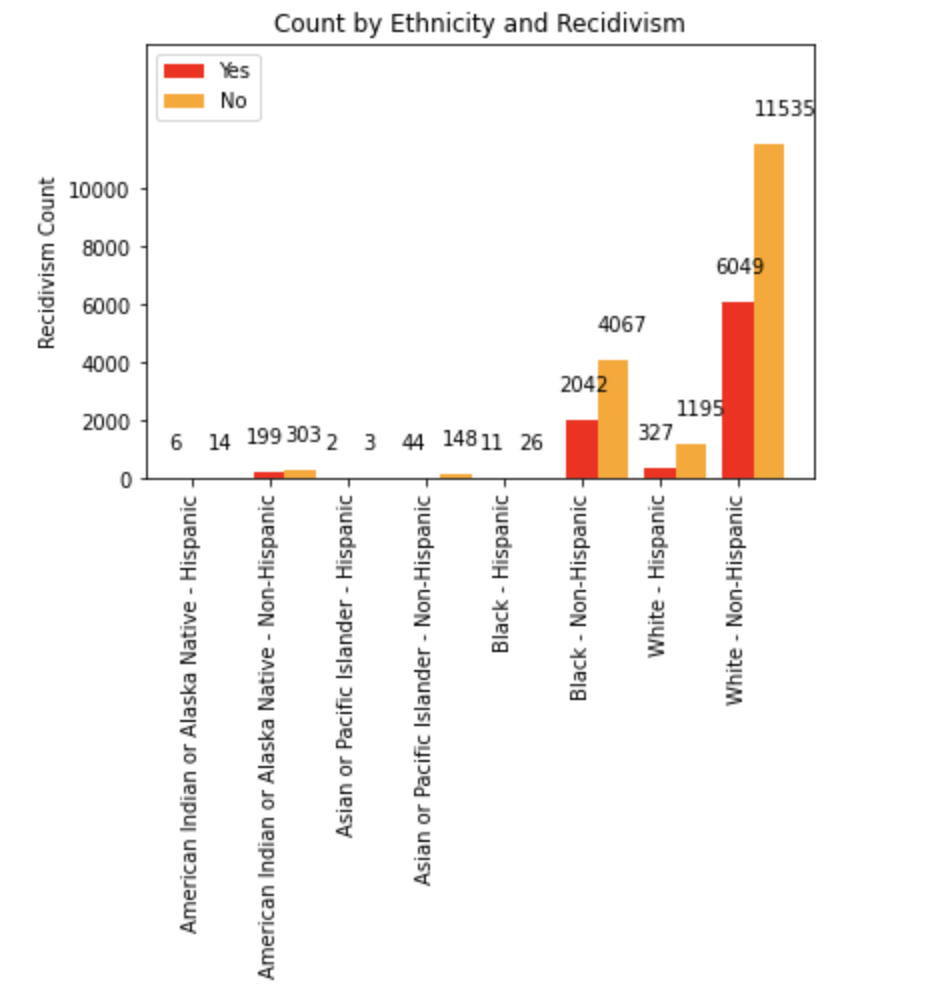
\includegraphics[width=3in]{1.png}
\caption{Data Distribution}
\end{figure}

\section{Models and Algorithms}

\hspace{5mm} We used sklearn’s decision tree as well as logistic regression packages to model the data. We created multiple models to predict both race and recidivism. When predicting for recidivism, we used both decision tree as well as logistic regression models. Models included and excluded race to check if race impacted recidivism predictions. When predicting for race, we used a decision tree with the recidivism feature.

In the decision tree models, a majority of the columns were binarized since the features were mainly categorical. After the transformation of the dataset into binarized values, the data is split into the testing and training sets before predicting recidivism.



\section{Results and Analysis}
Results and Analysis – Report on the accuracy or any evaluation metric you used. You may use
plots, graphs and
illustrations to describe your contributions.

\begin{figure}[h] 	
\centering
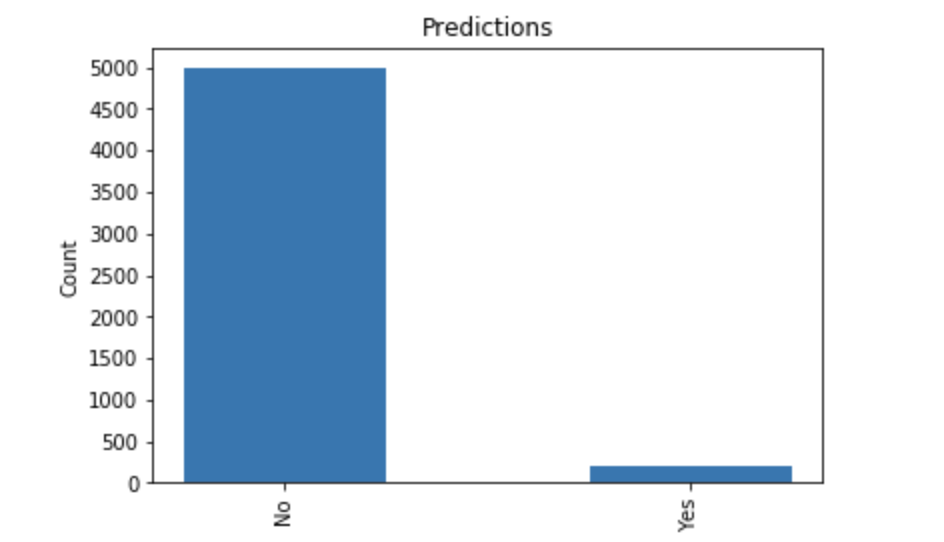
\includegraphics[width=3in]{2.png}
\caption{Without Race}
\end{figure}

\begin{figure}[h] 	
\centering
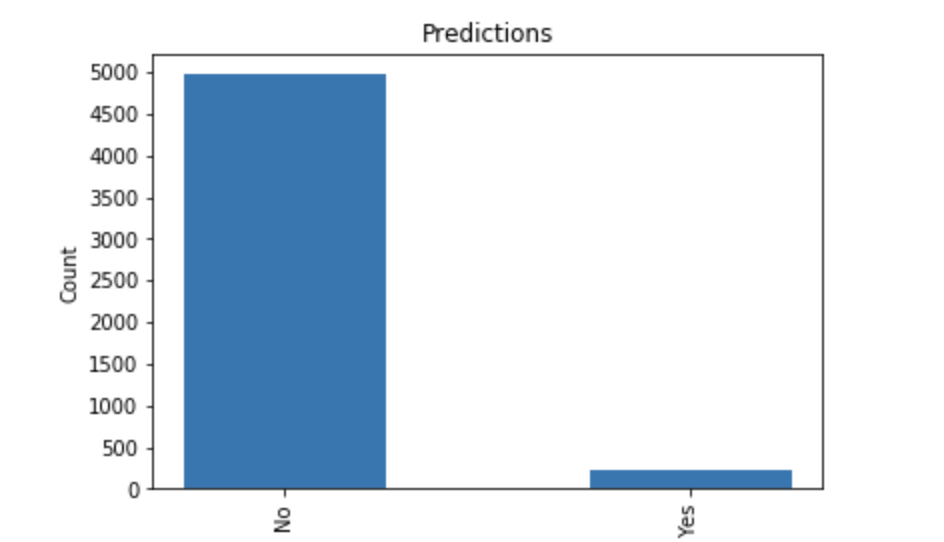
\includegraphics[width=3in]{3.png}
\caption{With Race}
\end{figure}

\begin{figure}[h] 	
\centering
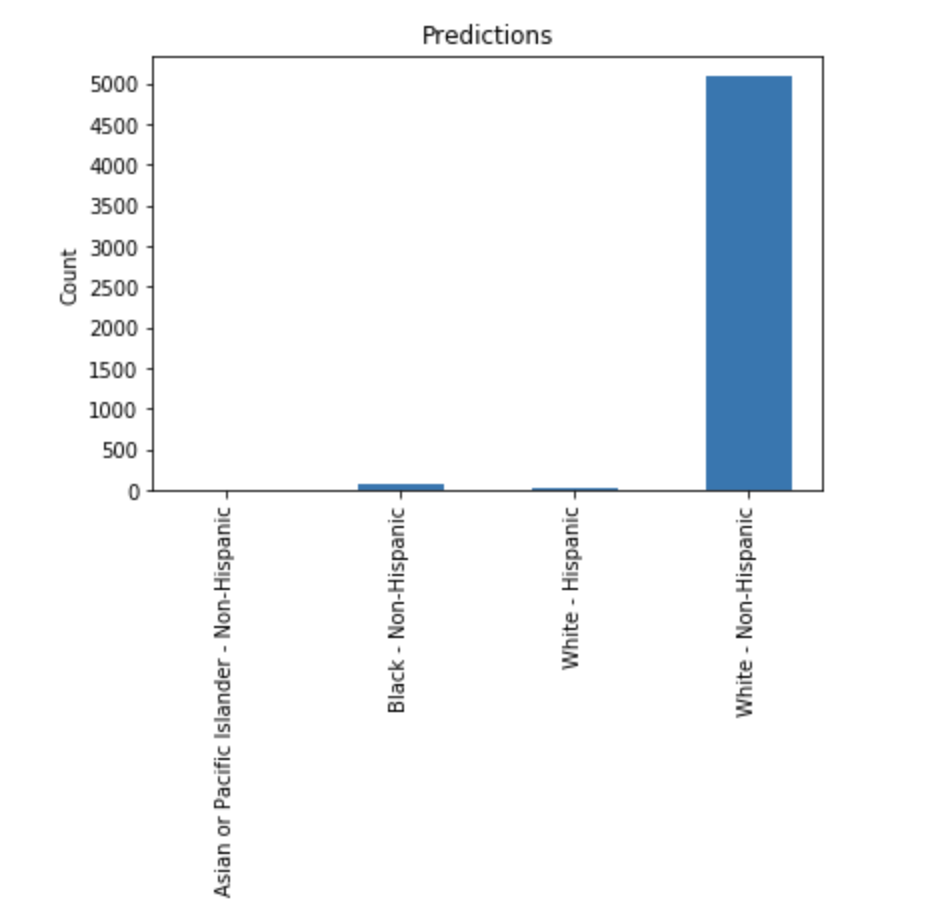
\includegraphics[width=3in]{4.png}
\caption{Predicting Race}
\end{figure}

\section{Contribution}
Contribution – Describe how each member of the team contributed to the final project.


\section{Future Work}
Future work – How could you foresee the project progressing if work were to continue in the
future?


Turn in report, zip file with any data, code (optional) by March 15 for your group.

\begin{thebibliography}{1}

\bibitem{1}
Angwin, Julia; Larson, Jeff (2016-05-23). "Machine Bias". ProPublica. Retrieved 2019-11-21.

\end{thebibliography}
\end{document}